\begin{center}
	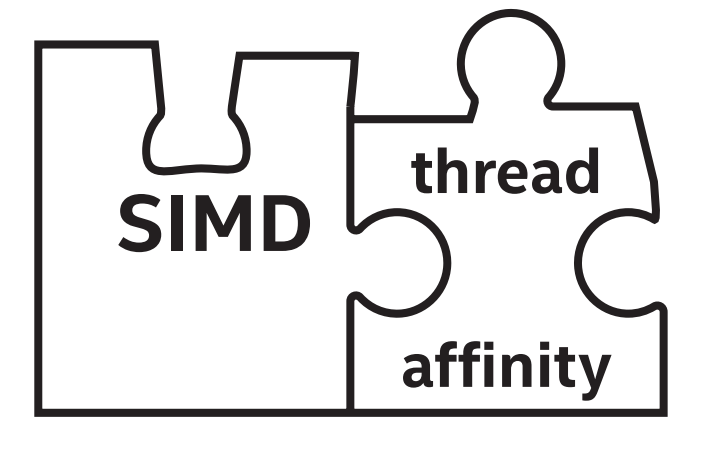
\includegraphics[width=0.3\textwidth]{content/chapter-16/images/1}
\end{center}

内核编程最初作为GPU编程的方式。由于是通用内核编程,理解编程风格如何影响代码向CPU的映射就很重要。\par

CPU在过去的几年里不断发展。在2005年左右发生了一个重大的变化,当时增加时钟速度带来的性能的提升减少了。并行性是最受欢迎的解决方案——CPU生产商引入了多核芯片,而不是提高时钟频率。计算机可以同时执行多个任务!\par

虽然多核是提高硬件性能的主流方式,但在软件上释放这种能力需要付出很大的努力。多核处理器要求开发人员对算法进行修改,这样硬件性能增益才会明显,但想要做到却很难。拥有的核芯越多,就越难高效地工作。DPC++是解决这些挑战的编程语言,有助于在CPU(和其他体系结构)上开发各种形式的并行。\par

本章讨论了CPU架构的一些细节,CPU硬件如何执行DPC++应用程序,并提供了在为CPU平台编写DPC++代码的最佳实践。\par






